%=======================================================Kapitola: Měniče s vnější komutací==========================================================
\chapter{Měniče s vnější komutací}
\minitoc
\newpage
  \section{Takt a komutace}
    Spínáním hlavních polovodičových součástek v \emph{hlavním obvodu} měniče nebo spínače je realizována žádaná funkce, tj. přeměna parametrů elektrické energie, u měničů, a spínání u spínačů. \emph{Vedlejší obvod}, včetně vedlejších polovodičových součástek, zajišťuje činnost hlavního obvodu (např. vypínání hlavních tyristorů). Každá část hlavního obvodu mezi dvěma uzly je \emph{hlavní větev}. Každá část vedlejšího obvodu mezi dvěma uzly je \emph{vedlejší větev}.

   \textbf{Takt} je časový interval mezi dvěma po sobě následujícími změnami vodivosti větví měniče či spínače. Označujeme jej značkami sepnutých součástek. Tak např. takt V1, V2 je časový interval, ve kterém jsou sepnuty součástky V1, V2.

   \textbf{Komutace} větví měniče (spínače) je elektromagnetický děj v obvodu měniče (spínače) charakterizovaný přechodem proudu z jedné větve měniče (spínače) na druhou aniž by byl přerušen proud odtékající z (nebo přitékající do) uzlu obou větví. Termín komutace měniče (spínače) nelze zaměňovat s termínem komutace polovodičové součástky. Ke komutaci běžné dochází po sepnutí polovodičové součástky jedné z komutujících větví, \emph{Sepnutí a nárůst proudu v této větvi, pokles proudu a nakonec vypnutí polovodičové součástky ve druhé větvi, umožňuje komutační napětí působící na obě větve}.

   \begin{figure}
     \centering
     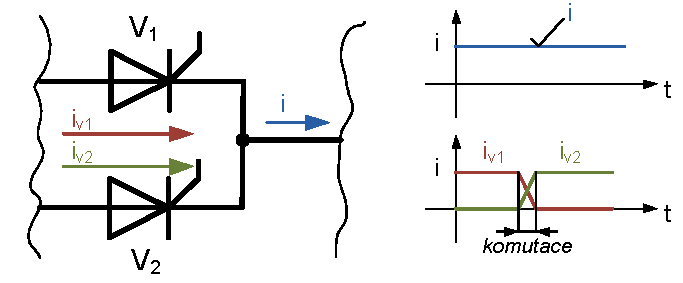
\includegraphics[scale=1]{komutace.pdf}
     \caption{Komutace.}
     \label{ve:fig_komutace}
   \end{figure}

   \begin{itemize}
     \item \textbf{Vnější komutace} (dříve označována jako přirozená komutace) se vyznačuje zdrojem komutačního napětí umístěným vně měniče. Užšími termíny síťová komutace nebo zátěžová komutace je blíže určován původ komutačního napětí.
     \item \textbf{Vlastní komutace} (dříve označována jako nucená komutace) se vyznačuje zdrojem komutačního napětí umístěným ve vlastním obvodu měniče.
     \item \textbf{Přímá komutace} probíhá v jednom komutačním taktu (obr. \ref{ve:fig_komutace}), přímo z jedné hlavní větve na druhou. Přímou komutaci je možno označit též jako jednostupňovou.
   \end{itemize}